\def\pgfsysdriver{pgfsys-dvisvgm.def}
% flashcards-title: Cue to response path with an interrupted link
% flashcards-desc: Four labeled boxes run from cue through detector and internal relay to response. A black X interrupts the link between detector and relay.
\documentclass[tikz,border=6pt]{standalone}
\usetikzlibrary{arrows.meta,calc,fit,positioning,shapes.geometric}

\definecolor{fcink}{HTML}{17212B}
\definecolor{fcblue}{HTML}{1D5D8C}
\definecolor{fcgreen}{HTML}{2D6A4F}
\definecolor{fcorange}{HTML}{A44A1F}
\definecolor{fcpale}{HTML}{F4F7F9}
\definecolor{fcsoil}{HTML}{8B5E3C}

\tikzset{
  fc text/.style={font=\sffamily, text=fcink},
  fc panel/.style={draw=fcink, line width=0.9pt, rounded corners=5pt, fill=fcpale},
  fc node/.style={draw=fcink, line width=0.9pt, rounded corners=4pt, fill=white,
    minimum width=24mm, minimum height=10mm, align=center, font=\sffamily},
  fc arrow/.style={-{Stealth[length=3.2mm,width=2.4mm]}, line width=1.2pt,
    draw=fcblue, line cap=butt},
  fc boundary/.style={draw=fcorange, line width=1.4pt, dash pattern=on 5pt off 3pt,
    rounded corners=7pt},
  fc label/.style={font=\sffamily\bfseries, text=fcink},
  fc note/.style={font=\sffamily\small, text=fcink, align=center}
}

\begin{document}
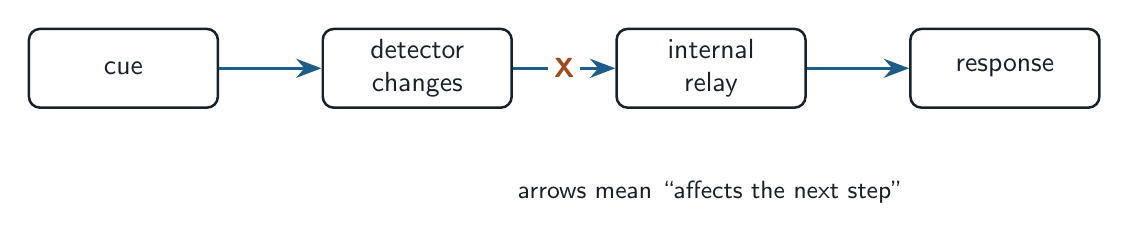
\begin{tikzpicture}[fc text, node distance=13mm]
  \node[fc node] (cue) {cue};
  \node[fc node, right=of cue] (det) {detector\\changes};
  \node[fc node, right=of det] (relay) {internal\\relay};
  \node[fc node, right=of relay] (resp) {response};
  \draw[fc arrow] (cue)--(det);
  \draw[fc arrow] (det)--(relay);
  \draw[fc arrow] (relay)--(resp);
  \node[fc label, text=fcorange, fill=white, inner sep=2pt] at ($(det)!0.5!(relay)$) {X};
  \node[fc note, below=8mm of relay] {arrows mean ``affects the next step''};
\end{tikzpicture}
\end{document}
